%TITULO-------------------------------------------------------------------

%=========================================================================
\chapter{Resultados}\label{resultados}
%=========================================================================

    A comprovação da teoria desenvolvida nos capítulos anteriores é feita através da demonstração de resultados de simulação e experimentais. As simulações são feitas utilizando o software \textsc{Matlab}, da empresa \textit{MathWorks}$^\circledR$. Mais especificamente, o \textit{toolbox} Simulink é o componente central para realizar as simulações. O filtro \textit{LCL} é descrito como uma função de transferência, o conversor e a fonte são simulados usando modelos disponíveis no Simulink. A plataforma \textsc{dSpace} serve como uma interface entre o circuito real e o \textsc{Matlab}, dispondo de $n_{ADs}$ conversores analógico-digitais (\emph{AD}) e $n_{DAs}$ conversores digitais-analógicos (\emph{DA}). São feitas medidas em tempo real no circuito e é feita a aquisição dessas medidas via \textsc{dSpace}. A plataforma se encarrega de disponibilizar as medidas adquiridas em um bloco do Simulink, onde podem ser utilizadas diretamente no cálculo da ação de controle. Uma vez computada, a ação de controle transcrita em comando de acionamento das chaves do conversor e então enviada via \emph{DA} para o conversor.

    Os resultados experimentais são obtidos utilizando uma bancada composta por uma fonte \textit{modelo}, um conversor \textsc{Semikron} \textit{modelo} e uma interface \textsc{dSpace} \textit{modelo}. A Fig.~\ref{fig:topologia_bancada} apresenta a disposição dos elementos da bancada.

    \begin{figure}[htb]
        \centering{
            %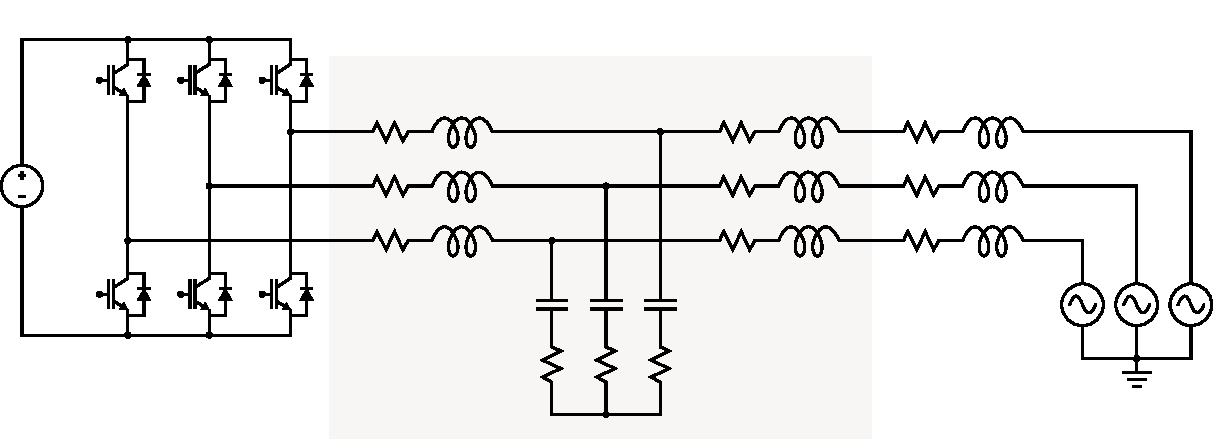
\includegraphics[width=0.9\textwidth]{img/topologia}}
            \def\svgwidth{0.9\textwidth}
            \input{./img/bancada.pdf_tex}}
        \renewcommand\figurename{Fig.}
        \caption{Diagrama que representa os elementos da bancada.}
        \label{fig:topologia_bancada}
    \end{figure}


\section{Resultados de Simulação}

	O Simulink dispõe de muitos blocos cujos modelos matemáticos são geralmente aceitos como precisos o suficiente para representar elementos do mundo real. Por isso, os modelos de conversor, linha de transmissão, transformador e fonte são utilizados neste trabalho para representar o comportamento de elementos reais.

	A ação de controle é implementada na simulação via código escrito em linguagem própria do \textsc{Matlab}, chamada \textit{linguagem .m}. Existe um bloco no Simulink chamado \textit{Subsystem}, que recebe sinais de entrada e permite que esses sinais sejam manipulados via código para gerarem sinais de saída. Este bloco é utilizado para implementar a ação de controle projetada nos capítulos anteriores.

	Como a simulação é implementada em tempo discreto, os principais passos realizados são os seguintes:

	\begin{enumerate}
		\item \textit{Inicialização}: no início da simulação, são carregados os valores iniciais para as variáveis;
		\item \textit{Amostragem das variáveis}: as variáveis são amostradas para a realização dos cálculos preliminares da ação de controle;
		\item \textit{Cálculo da ação de controle}: a ação de controle é calculada e tornada disponível, e o estado atual das variáveis é armazenado como sendo o estado anterior para a próxima iteração da simulação;
		\item \textit{Geração da saída}: a ação de controle é aplicada ao sistema e a saída é atualizada de acordo.
	\end{enumerate}

	A Fig.~\ref{fig:i2_simulacao} apresenta a corrente da rede em comparação com a referência. No instante $t_1$ ocorre inversão de fase na referência. No instante $t_2$ é aplicado um degrau de amplitude na referência. No instante $t_3$ é realizada uma variação na indutância da rede.

	\begin{figure}[htb]
        \centering{
            %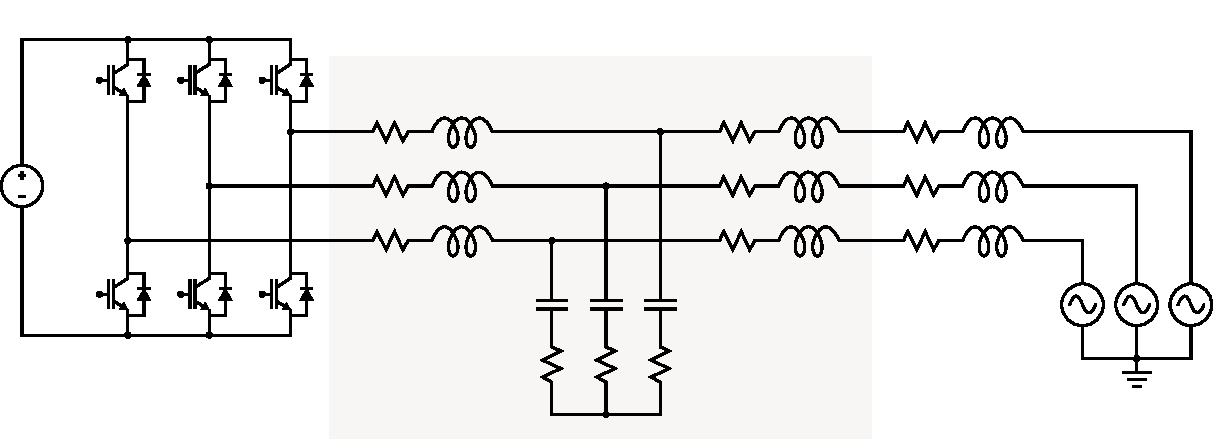
\includegraphics[width=0.9\textwidth]{img/topologia}}
            \def\svgwidth{0.6\textwidth}
            \input{./img/logo.pdf_tex}}
        \renewcommand\figurename{Fig.}
        \caption{Corrente da rede $i_2$ em relação à referência.}
        \label{fig:i2_simulacao}
    \end{figure}

\section{Resultados Experimentais}



%FIM----------------------------------------------------------------------
